\section{Swarm Fusion Method}
\yasu{need to polish, reads very bad.}  Swarm Fusion is a natural
parallel extension of Fusion Move Method. Take a multi-threading
environment to explain our idea, which is also applicable to other
parallel computation environments such as cloud computing. Assume we
have $N$ threads $\{T_i | i=1, 2, \cdots, N\}$. There are two places to
collect solutions or solution proposals for fusion. First, the {\it
proposal pool} can generate new solution proposals on request.
%
Second, the {\it solution pool} stores the solutions that have been
fused by the threads. At default, each thread keeps only a current
solution in the pool, but the scheme can be more general. Two
parameters $\alpha_i$ and $\beta_i$ control the behavior of each fusion
step in $T_i$. The thread collects $\alpha_i$ solution proposals
from the proposal pool and $\beta_i$ solutions from the solution pool
for fusion in each step.
%
Furthermore, one can also control how to choose proposal generation
schemes and/or solutions from the pools.

\mysubsubsection{Base architecture}
The swarm fusion is highly flexible, and we first introduce our base
architecture that exploits general strenghts offered by the
framework. Later, we explain how to further optimize the configuration
to boost performance for specific problems. In the base architecture,
all the threads fuse some number of proposals from the proposal pool and
some number of solutions from the solution pool in each step. In other
words, all the threads constantly exchange solutions while injecting new
proposals. This architecture is illustrated in Figure~\ref{fig:base}.

\begin{figure}[tb]
 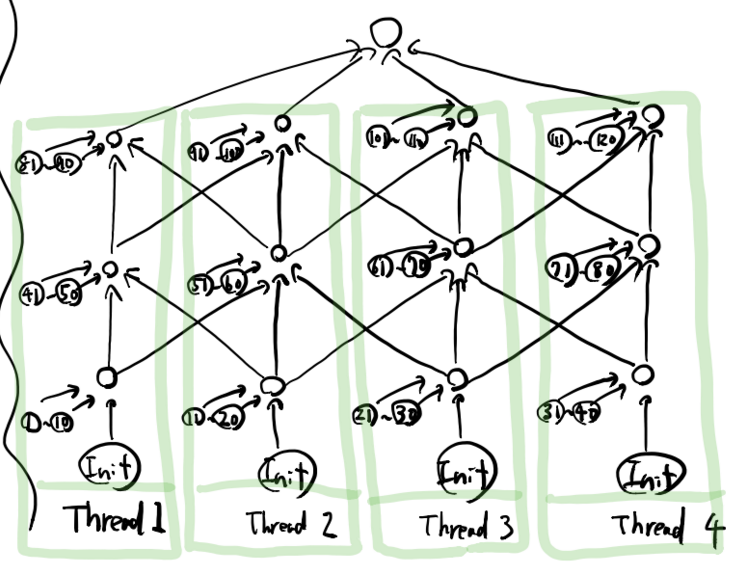
\includegraphics[width=\columnwidth]{figure/base_illustration.png}
 \caption{Base Swarm Fusion architecture.}\label{fig:base}
\end{figure}

\mysubsubsection{Relationships to existing methods} Our framework is
general, and it is easy to verify that existing parallel fusion
algorithms are just our special cases.
%
For example, the parallel fusion algorithm by Lempitsky et
al.~\cite{viktor} always performs binary fusion between the current
solution and another label, which can be achieved by setting $\alpha_i =
1$ and $\beta_i = 0$ for all the threads. The algorithm by
Veksler~\cite{olga} or Dejong et al.~\cite{dejong} hierarchically fuses
solutions starting from solution proposals. The algorithm can be
realized by setting $\alpha_i = 1, \beta_i = 0$ initially, then use
$\alpha_i = 0, \beta_i=1$  for the rest of the algorithm.

\noindent
We now illustrate the power of Swarm Fusion framework for three problems
in Computer Vision. 


% Suppose $N=4$, $\alpha_1 = 2$, and $\beta_1 = 3$. In this
% configuration, the first thread $T_1$ fuses its current solution $S_1$,
% two new proposal solutions (e.g., by randomly picking two proposal
% generation schemes), and the current solutions $(S_2, S_3, S_4)$ in the
% other three threads. This is a multi-way fusion with a non-submodular
% energy in general, and message passing algorithm such as
% TRW~\cite{kolmogorov} can be used. Sequential QPBO application is
% another.


% Our model is flexible. For example, a parallel fusion move algorithm by
% Lempitsky et al.~\cite{viktor} is a special case of ours, where $\alpha_i$

% , and it is easy to see that 
% Existing parallel fusion techniques are special 

% Our model is flexible and 
